

\section{Permutations By $k$ Inversions}
In the previous section we looked at permutation listings for all $n!$ permutations. In this section we look at 
listings for permutations by a given number of inversions. Let $k$ be the number of inversions for a given permutation 
of order $n$. Let $\Pi_{n,k}$ indicate the number of permutations of order $n$ with $k$ inversions. We note that the $\Pi_{n,k}$ is counted by 
the triangle of Mahonian numbers~\cite{A40}. Let \emph{$S_{n,k}$} denote all permutations of order $n$ with $k$ inversions. 
%%Paragraph 
\subsection{Effler-Ruskey Algorithm}
%%%%%%%%%%FIX ME %%%%%%%%%%%%%%%%
In the paper A CAT Algorithm for Generating Permutations with a Fixed Number of Inversions~\cite{A26}, 
written by Effler and Ruskey, the authors provide a constant amortized time algorithm for 
generating all permutations of order $n$ with $k$ inversions. 
The algorithm is also a \emph{BEST} algorithm (backtracking ensures success at terminals), meaning that when the algorithm backtracks, 
the back-tracking leads to a successful result. We define the \emph{empty permutation of order $n$} as an empty 
vector of length $n$.
Let the initial conditions of the algorithm be the following. Let $\pi$ be the empty permutation of order $n$. 
Let $k$ be initialized to an integer between $[0 \dots {n \choose 2}]$. 
Let $list$ be initialized to the list of $n$ elements in strictly ascending order. 
Let $i$ be the index of element $x$ in $list$, using one indexing. $n-i$ 
indicates the number of inversions formed with $x$ when inserting $x$ into position $n$ in $\pi$.
The algorithm works as follows.
Going right to left in the $list$, each element $x$ is inserted into $p_{n}$
only if inserting $x$ into position $n$ in $\pi$ does not exceed the current number of inversions, $k$. I.e. only 
if $k- (n-i)\geq 0$.
If $x$ is inserted into $\pi$ at position $n$ then $x$ is removed from $list$, a recursive call is made such that $n$ is reduced by 
$1$ and $k$ is reduced by $(n-i)$. When the function returns from its recursive call, element $x$ is placed back into the list 
at its original position. To see the algorithm please refer to Algorithm~\ref{Alg:KInv}.
\begin{algorithm}[t]
    \begin{algorithmic}[1]
        \Function{KInversions}{$\pi$, $n$, $k$, $list$}
            \If{$n = 0$ and $k = 0$}
                \State {\sc Print}($\pi$)
            \Else
                \For{$i$ \textbf{from} length \textbf{of} $list$ \textbf{to} $1$}
                    \State $x \gets list_{i}$
                    \If{$n-i \leq k \leq {n-1\choose k} + (n-i)$}
                        \State $p_{n} \gets x$
                        \State remove $x$ from $list$ 
                        \State $k \gets k - (n-i)$
                        \State {\sc KInversions}$(\pi, n-1, k, list)$
                        \State insert $x$ in $list$ at correct position.
                    \EndIf
                \EndFor
            \EndIf
        \EndFunction
        
    \end{algorithmic}
    \caption{Generate all permutations with $k$ inversions}
    \label{Alg:KInv}
\end{algorithm} 

Below is an example of how the algorithm creates one permutation of order $4$ with $2$ inversions.
\begin{enumerate}
    \item Initial Call: {\sc KInversions}($\pi$=(\underline{ },\underline{ },\underline{ },\underline{ }),$n=4$,$k=2$,$list=[1,2,3,4]$):\newline 
    given $\pi$=(\underline{ },\underline{ },\underline{ },\underline{ }), $n=4$, $k=2$, $list=[1,2,3,4]$, $i=2$ and $x=3$ 
    then inserting $x$ into position $n=4$ would form $4-3=1$ 
    inversion(s). Specifically, the inversion $(4,3)$. Thus, $k$ would be reduced by $1$ in the recursive call 
    and $n$ would be reduced by $1$ in the recursive call. 

    \item First recursive call: {\sc KInversions}($\pi$=(\underline{ },\underline{ },\underline{ },\underline{3}),$n=3$,$k=1$,$list=[1,2,4]$):\newline 
    given $\pi$=(\underline{ },\underline{ },\underline{ },\underline{3}),$n=3$,$k=1$,$list=[1,2,4]$,$i=3$ and $x=4$
    then inserting $x$ into position $3$ would form $3-3=0$ inversions. Thus, $k$ would be reduced by $0$ in the 
    recursive call and $n$ would be reduced by $1$ in the recursive call.

    \item Second recursive call: {\sc KInversions}($\pi$=(\underline{ },\underline{ },\underline{4},\underline{3}),$n=2$,$k=1$,$list=[1,2]$):\newline 
    given $\pi$=(\underline{ },\underline{ },\underline{4},\underline{3}),$n=2$,$k=1$,$list=[1,2]$,$i=1$ and $x=1$
    then inserting $x$ into position $1$ would form $2-1=1$ inversion. Thus, $k$ would be reduced by $1$ to $0$ in the 
    recursive call and $n$ would be reduced by $1$ in the recursive call.

    \item Third recursive call: {\sc KInversions}($\pi$=(\underline{ },\underline{1},\underline{4},\underline{3}),$n=1$,$k=0$,$list=[2]$):
    \newline given $\pi$=(\underline{ },\underline{1},\underline{4},\underline{3}), $n=1$, $k=0$, $list=[2]$ $i=1$ and $x=2$
    then inserting $x$ into position $1$ would form $1-1=0$ inversions. Thus, $k$ would be reduced by $0$
    and $n$ would be reduced by $1$.

    \item Fourth recursive call: {\sc KInversions}($\pi$=(\underline{2},\underline{1},\underline{4},\underline{3}),$n=0$,$k=0$,$list=[]$):\newline 
    Given $n=0$ and $k=0$ the algorithm {\sc Prints}($\pi$) and returns.
\end{enumerate}

\subsection{Walsh} 
Despite the efficiency of Effler-Ruskey's algorithm, we note that the permutations are not listed in Gray code order. Therefore, we 
also look at the paper, Loop Free Sequencing of Bounded Integer Compositions, written by Walsh~\cite{A41}. Walsh provides an algorithm for listing 
$S_{n,k}$ in Gray code order in $0(1)$ time per permutation.  
Let an \emph{$n$ part composition of a non negative integer k} is an ordered n-tuple, $(g_{1},g_{2}  \dots ,g_{n})$, whose 
sum adds to $k$.
Such a composition is said to be $(m_{1},m_{2}, \dots m_{n})$ bounded when $0 \leq g_{i} \leq m_{i}$. Let $\pi$ be 
of order $n+1$, then we say $g$ is an n-tuple from $g_{1} \dots g_{n}$. We say $m$ is a bound on $g$ from 
$m_{1} \dots m_{n}$ such that each $m_{i}=min(n+1 - i, k)$ where $k$ is the target number of 
inversions. Each $g_{i}$ is bounded by $0 \leq g_{i} \leq m_{i}$. Let $g_{i}$ represent the 
number of inversions formed by placing an element from $[1 \dots n+1] \in \pi$ 
at index $i$ in $\pi$. We note that placing $1$ and index $1$ forms $0$ inversions and we note that 
placing $n+1$ at index $1$ forms $n$ inversions. $g$ is known as the inversion vector of $\pi$, bounded by $m$.\par 
Walsh lists $S_{n,k}$ by incrementing some $g_{i}$ by $1$ and decrementing some $g_{j}$ by $1$. Let $x$ and $y$ be positive integers indicating 
offsets from an index. Incrementing $g_{i}$ 
by $1$ induces a transposition in $\pi$ with $p_{i}$ and some element, $p_{i+x}$ in the suffix $p_{i+1} \dots p_{n+1}$, such that 
$p_{i} < p_{i+x} \wedge p_{i+x} < \forall p_{i+y}>p_{i}$. Decrementing $g_{j}$ by $1$ induces a transposition in 
$\pi$ with $p_{j}$ and some element, $p_{j+x}$ in the suffix $p_{j+1} \dots p_{n+1}$, such that $p_{j} > p_{j+x} \wedge p_{j+x} > \forall p_{j+y}<p_{j}$. 
We call $i$ the \emph{first pivot} $j$ the \emph{second pivot}, indicating that the increment occurs before the decrement; each pivot is found in 
$O(1)$ time. In Figure~\ref{Fig:Perm5,5}~\cite{A41}, all compositions, and permutations of order $5$ with $5$ inversions, are listed in the Gray code order 
found in Walsh's paper. In Chapter 5, by borrowing from Walsh's paper, we derive a Gray code for listing all ladders with $n$ lines and $k$ bars. 
\begin{figure}
    \centering 
    \resizebox{.4\textwidth}{.5\textwidth}{
            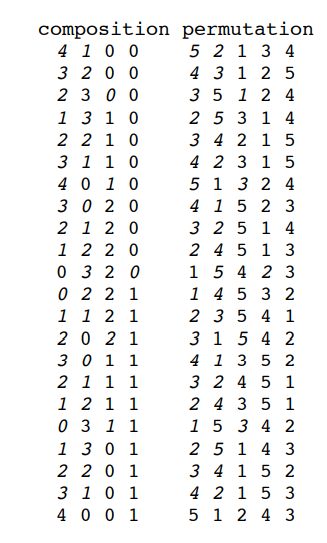
\includegraphics{Perm55}
    }
    \caption{Walsh's Gray code ordering of inversion vectors and corresponding permutations}
    \label{Fig:Perm5,5}
\end{figure}